% Cápitulo 3

\chapter{Un'architettura per la Rete Mocambos}
\label{Capitolo3}
\lhead{C\'apitulo 3. \emph{Uma arquitetura para Rede Mocambos}}

\section{Especificação dos requisitos}
A Rede Mocambos atualmente envolve cerca de 200 comunidades
localizadas em todo o território nacional brasileiro e algumas
comunidades na Africa e na Europa. A conectividade no Brasil é por
satélite, garantida pelo GESAC que disponibiliza para cada comunidade
uma \emph{Very Small Aperture Terminal} (VSAT) com banda de 512 kbit/s
em download e 128 kbit/s em upload. A topologia da rede é a estrela
então todos os nós comunicam por satélite concentrando o trafego num
\emph{hub} terrestre, onde a rede via satélite é interligada a
Internet. Cada comunidade tem uma sala com 10 computadores com acesso
publico, recém instalados (ou sendo instalados) pelo
Telecentros.BR\footnote{``O Programa Nacional de Apoio à Inclusão
  Digital nas Comunidades – Telecentros.BR é uma ação do Governo
  Federal de apoio à implantação de novos espaços públicos e
  comunitários de inclusão digital e o fortalecimento dos que já estão
  em funcionamento em todo o território. São disponibilizados
  equipamentos de informática e mobiliário necessários ao
  funcionamento dos telecentros, serviços de conexão em banda larga à
  internet, assim como a formação e bolsas de auxílio financeiro para
  monitores atuarem como agentes de inclusão digital. Esses monitores
  bolsistas participam de um curso de formação e atendem as
  comunidades dos telecentros.'', retirado de
  \url{http://www.inclusaodigital.gov.br/telecentros}.}, outro
programa do governo federal. A população de casa comunidade varia
desde as centenas as milhares de pessoas. A maioria das comunidade se
encontra em área rural, geralmente de difícil acesso e sem outros
meios de comunicação. Além dos espaços comunitários, normalmente
concentrados na zona central, a população é dividida em pequenos
núcleos familiares espalhados no território e as vezes muito distantes
um dos outros.

Vejamos agora alguns requisitos essenciais para essa arquitetura de
rede federada.

\subsection{Identidade de rede}
Os usuários das comunidades tem que ter identidade digitais com as
quais acessar e usar os serviços existentes. Além de acessar
localmente, é importante ter acesso a alguns serviços também fora da
própria comunidade. Por exemplo, no caso uma pessoa se encontra na
cidade, ela deve poder acessar, através da internet, aos serviços de
base, como o e-mail, o aos portais e serviços web da RM. É necessária
então uma identidade digital de rede univoca. 

\subsection{Autenticação descentralizada}
\label{sec:AutDec}
Um requisito essencial para cada comunidade é ter autonomia em
ausência de conexão internet, e a presença então de um sistema local
de autenticação e autorização. Além de garantir a continuidade do
serviço (em relação a problemas da conexão por satélite), é um
requisito importante para um bom desempenho de todos os serviços autenticados. 

\subsection{Sincronização}\label{Sincronizazzione}
A troca de informações entre as comunidades é o objetivo primário para
a RM. É então necessário um sistema para a sincronização seletiva dos
conteúdos de interesse geral. Para otimizar o uso da banda, as
operações de sincronização dos dados tem que influenciar o minimo
possível o uso quotidiano da internet, programando essas operações
durante a noite o de qualquer forma quando a conexão por satélite não
ta sendo usada. 

\subsection{Replicabilidade}
Cada comunidade se organiza autonomamente para a gestão da própria
infraestrutura tecnológica e as soluções adotadas tem então que ser
facilmente implementáveis e adaptáveis localmente. As ferramentas
precisam ser então soluções estáveis e possivelmente de uso comum,
também ao fim de encontrar mais facilmente assistência em loco. 

\subsection{Manutenção}
A manutenção do sistema tem que prever seja intervenções a distancia
seja locais. O sistema é baseado em tecnologias \emph{standard} e
abertas para garantir o acesso aos dados mesmo em caso de problemas.

\subsection{Desenvolvimento}
Cada comunidade tem características e necessidades próprias que levam
a serviços diferenciados. A arquitetura geral da RM tem que ser uma
base estável em cima da qual poder desenvolver sem demais restrições.
As tecnologias e as linguagens adotadas tem que facilitar a interação,
a formação e o reuso dos conhecimentos. 


======================================================================



\section{Strumenti e pratiche per lo sviluppo}
Data la natura della RM, e in particolare la necessità di autonomia
tecnologica, la formazione è fondamentale per cui è importante l'uso
di strumenti che facilitino la documentazione e lo sviluppo
collettivo. La RM utilizza già da anni un wiki\footnote{``Una Wiki è
  una pagina (o comunque una collezione di documenti ipertestuali) che
  viene aggiornata dai suoi utilizzatori e i cui contenuti sono
  sviluppati in collaborazione da tutti coloro che vi hanno
  accesso. La modifica dei contenuti è aperta, nel senso che il testo
  può essere modificato da tutti gli utenti (a volte soltanto se
  registrati, altre volte anche anonimi) contribuendo non solo per
  aggiunte come accade solitamente nei forum, ma anche cambiando e
  cancellando ciò che hanno scritto gli autori precedenti.  Ogni
  modifica è registrata in una cronologia che permette in caso di
  necessità di riportare il testo alla versione precedente; lo scopo è
  quello di condividere, scambiare, immagazzinare e ottimizzare la
  conoscenza in modo collaborativo. Il termine wiki indica anche il
  software collaborativo utilizzato per creare il sito web e il
  server.'', tratto da \url{http://it.wikipedia.org/wiki/Wiki}.},
disponibile all'indirizzo \url{http://wiki.mocambos.net}, dove è
disponibile, in lingua portoghese, una parte della documentazione sul
codice sviluppato per questo lavoro. Per il \emph{versionamento} del
codice del lavoro svolto si è scelto di usare il sistema decentrato
GIT (vedi \ref{sec:GIT}) e la piattaforma
GITHUB\footnote{\href{http://github.com}{GITHUB} è una rete sociale
  basata sul sistema GIT \ref{sec:GIT}.}. Il codice del prototipo è
disponibile all'indirizzo \url{https://github.com/RedeMocambos}

\subsection{Sistema operativo}
La scelta di un sistema operativo comune facilita la documentazione,
l'automazione e l'assistenza a distanza. Molte comunità utilizzano già
distribuzioni GNU/Linux basate su Debian\footnote{``Il Progetto Debian
  è una associazione di persone che ha come scopo comune la creazione
  di un sistema operativo libero. Il sistema operativo che abbiamo
  creato si chiama Debian GNU/Linux, o semplicemente Debian.'', tratto
  da \url{http://www.debian.org/}}. Per il prototipo sono state scelte
l'ultima versione stabile, di Debian, la 6.0, e di
Ubuntu\footnote{``Ubuntu è un sistema operativo GNU/Linux nato nel
  2004, basato su Debian, che si focalizza sull'utente e sulla
  facilità di utilizzo. Ubuntu è orientato all'utilizzo desktop e pone
  una grande attenzione al supporto hardware. È prevista una nuova
  versione ogni sei mesi.  Finanziato dalla società Canonical Ltd
  (registrata nell'Isola di Man), questo sistema è rilasciato come
  software libero sotto licenza GNU GPL ed è gratuito e liberamente
  modificabile.'', tratto da
  \url{http://it.wikipedia.org/wiki/Ubuntu}.}, la 11.10.

\subsection{Linguaggi di programmazione}
Per il sistema sviluppato si è scelto l'uso del linguaggio di
programmazione Python, un linguaggio molto flessibile e probabilmente
il più versatile per connettere componenti eterogenee. Inoltre alcune
comunità già usano Software Liberi, quali
\emph{GIMP}\footnote{\emph{GNU Image Manipulation Program (GIMP)} è un
  programma per il fotoritocco, montaggio e creazione di
  immagini. Disponibile su \url{http://www.gimp.org/}.},
\emph{Blender}\footnote{\emph{Blender} è un programma per la creazione
  di grafica e ambienti tridimensionali. Disponibile su
  \url{http://www.blender.org/}.},
\emph{Inkscape}\footnote{\emph{Inkscape} è un programma di grafica
  vettoriale conforme allo standard SVG. Disponibile su
  \url{http://inkscape.org}.} che fanno ampio uso di \emph{scripting}
Python per la creazione di filtri e per altre funzionalità avanzate.

\subsection{Virtualizzazione}
Il prototipo è stato sviluppato e testato in un ambiente
virtualizzato, per garantire maggior controllo e verificare la
correttezza del procedimento in tutti i suoi passaggi. Gli
\emph{script} per automatizzare le installazioni, e le procedure passo
passo presenti nella documentazione, sono state eseguite a partire da
un sistema base. Sono state create delle macchine virtuali, con
l'aiuto del programma libero
\emph{VirtualBox}\footnote{\emph{VirtualBox} è un virtualizzatore
  completo per architettura x86 per l'uso in server, computer
  personali e sistemi \emph{embedded}. Dispobibile su
  \url{http://www.virtualbox.org/}.}, simulando dei server
comunitari/locali e il server centrale.


\section{Architettura di base}

\subsection{Gestione delle identità di rete}
Analizzando la specifica dei requisiti e alcune delle tecnologie
esistenti viste nel capitolo precedente, è stato scelto l'uso di LDAP
per gestire le credenziali degli utenti all'interno della RM. Il
prototipo proposto prevede un server centrale su connettività internet
garantita e server locali in replica. È possibile pensare una
configurazione in cui tutti i server della rete sono configurati in
modalità N-Way-Multimaster. Questa configurazione, se da un lato
consente l'aggiornamento in scrittura della base utenti su ognuno dei
server, può generare più facilmente situazioni di inconsistenza dei
dati e problemi di sincronizzazione tra i server LDAP. Per questo
motivo per il prototipo realizzato si è scelto di rilassare il
requisito \ref{sec:AutDec}, ipotizzando un singolo server master per
tutta la rete su cui effettuare le operazioni in scrittura (creazione,
eliminazione e aggiornamento di utenti) e server locali abilitati solo
ad operazioni in lettura. Ogni comunità quindi avrebbe a disposizione
un server LDAP in replica su cui basare le operazioni di
autenticazione e autorizzazione. In mancanza di connessione esterna i
servizi locali rimangono comunque attivi per le utenze attive fino
all'ultima sincronizzazione.


\subsection{Mocambos\_LDAP}\label{MocambosLDAP}
\framebox[\textwidth]{\footnotesize Il codice è disponibile su
\url{https://github.com/RedeMocambos/Mocambos_LDAP}}

Per facilitare l'implementazione dei server LDAP dagli amministratori
locali è stato sviluppato uno script di installazione, che può tornare
utile anche per un amministratore remoto.

Lo script \textit{bash} provvede ad installare i pacchetti necessari e
preparare il server LDAP \emph{slapd} in configurazione master o
replica. Inoltre crea un DIT preconfigurato per la RM con una semplice
struttura (vedi figura \ref{fig:DIT_ReteMocambos}).

\begin{figure}[htbp]
  \centering
  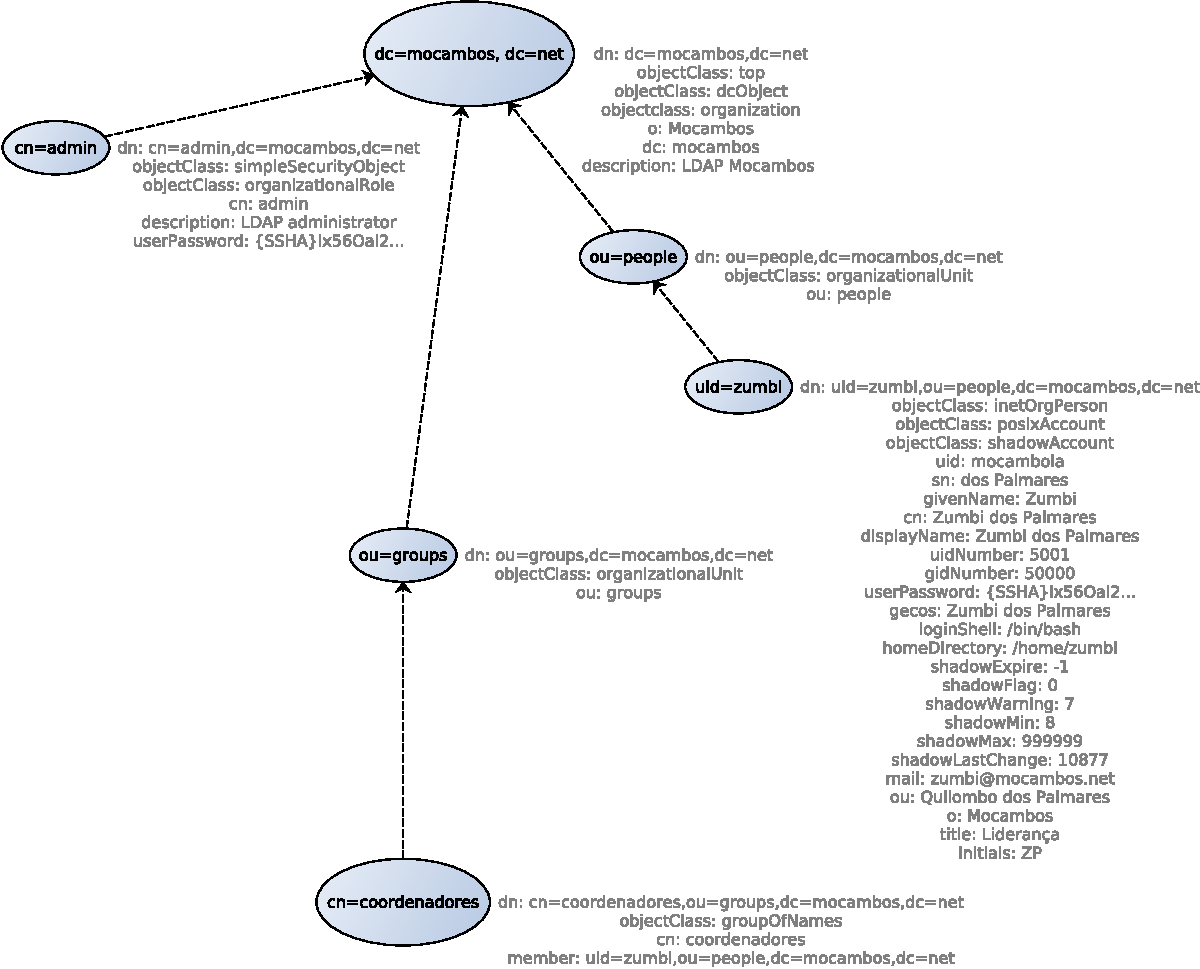
\includegraphics[width=\textwidth]{./Figure/DIT_ReteMocambos-crop.pdf}
  \rule{35em}{0.5pt}
  \caption[DIT di base del server LDAP della RM]{DIT di base del
    server LDAP della RM.}
  \label{fig:DIT_ReteMocambos}
\end{figure}




